\documentclass[../Draft_harmonization_paper.tex]{subfiles}

\begin{document}

\section*{Supporting Information}

\subsection*{Comparison of the trait aggregation methods with each other}

\begin{figure}[H]
    \centering
    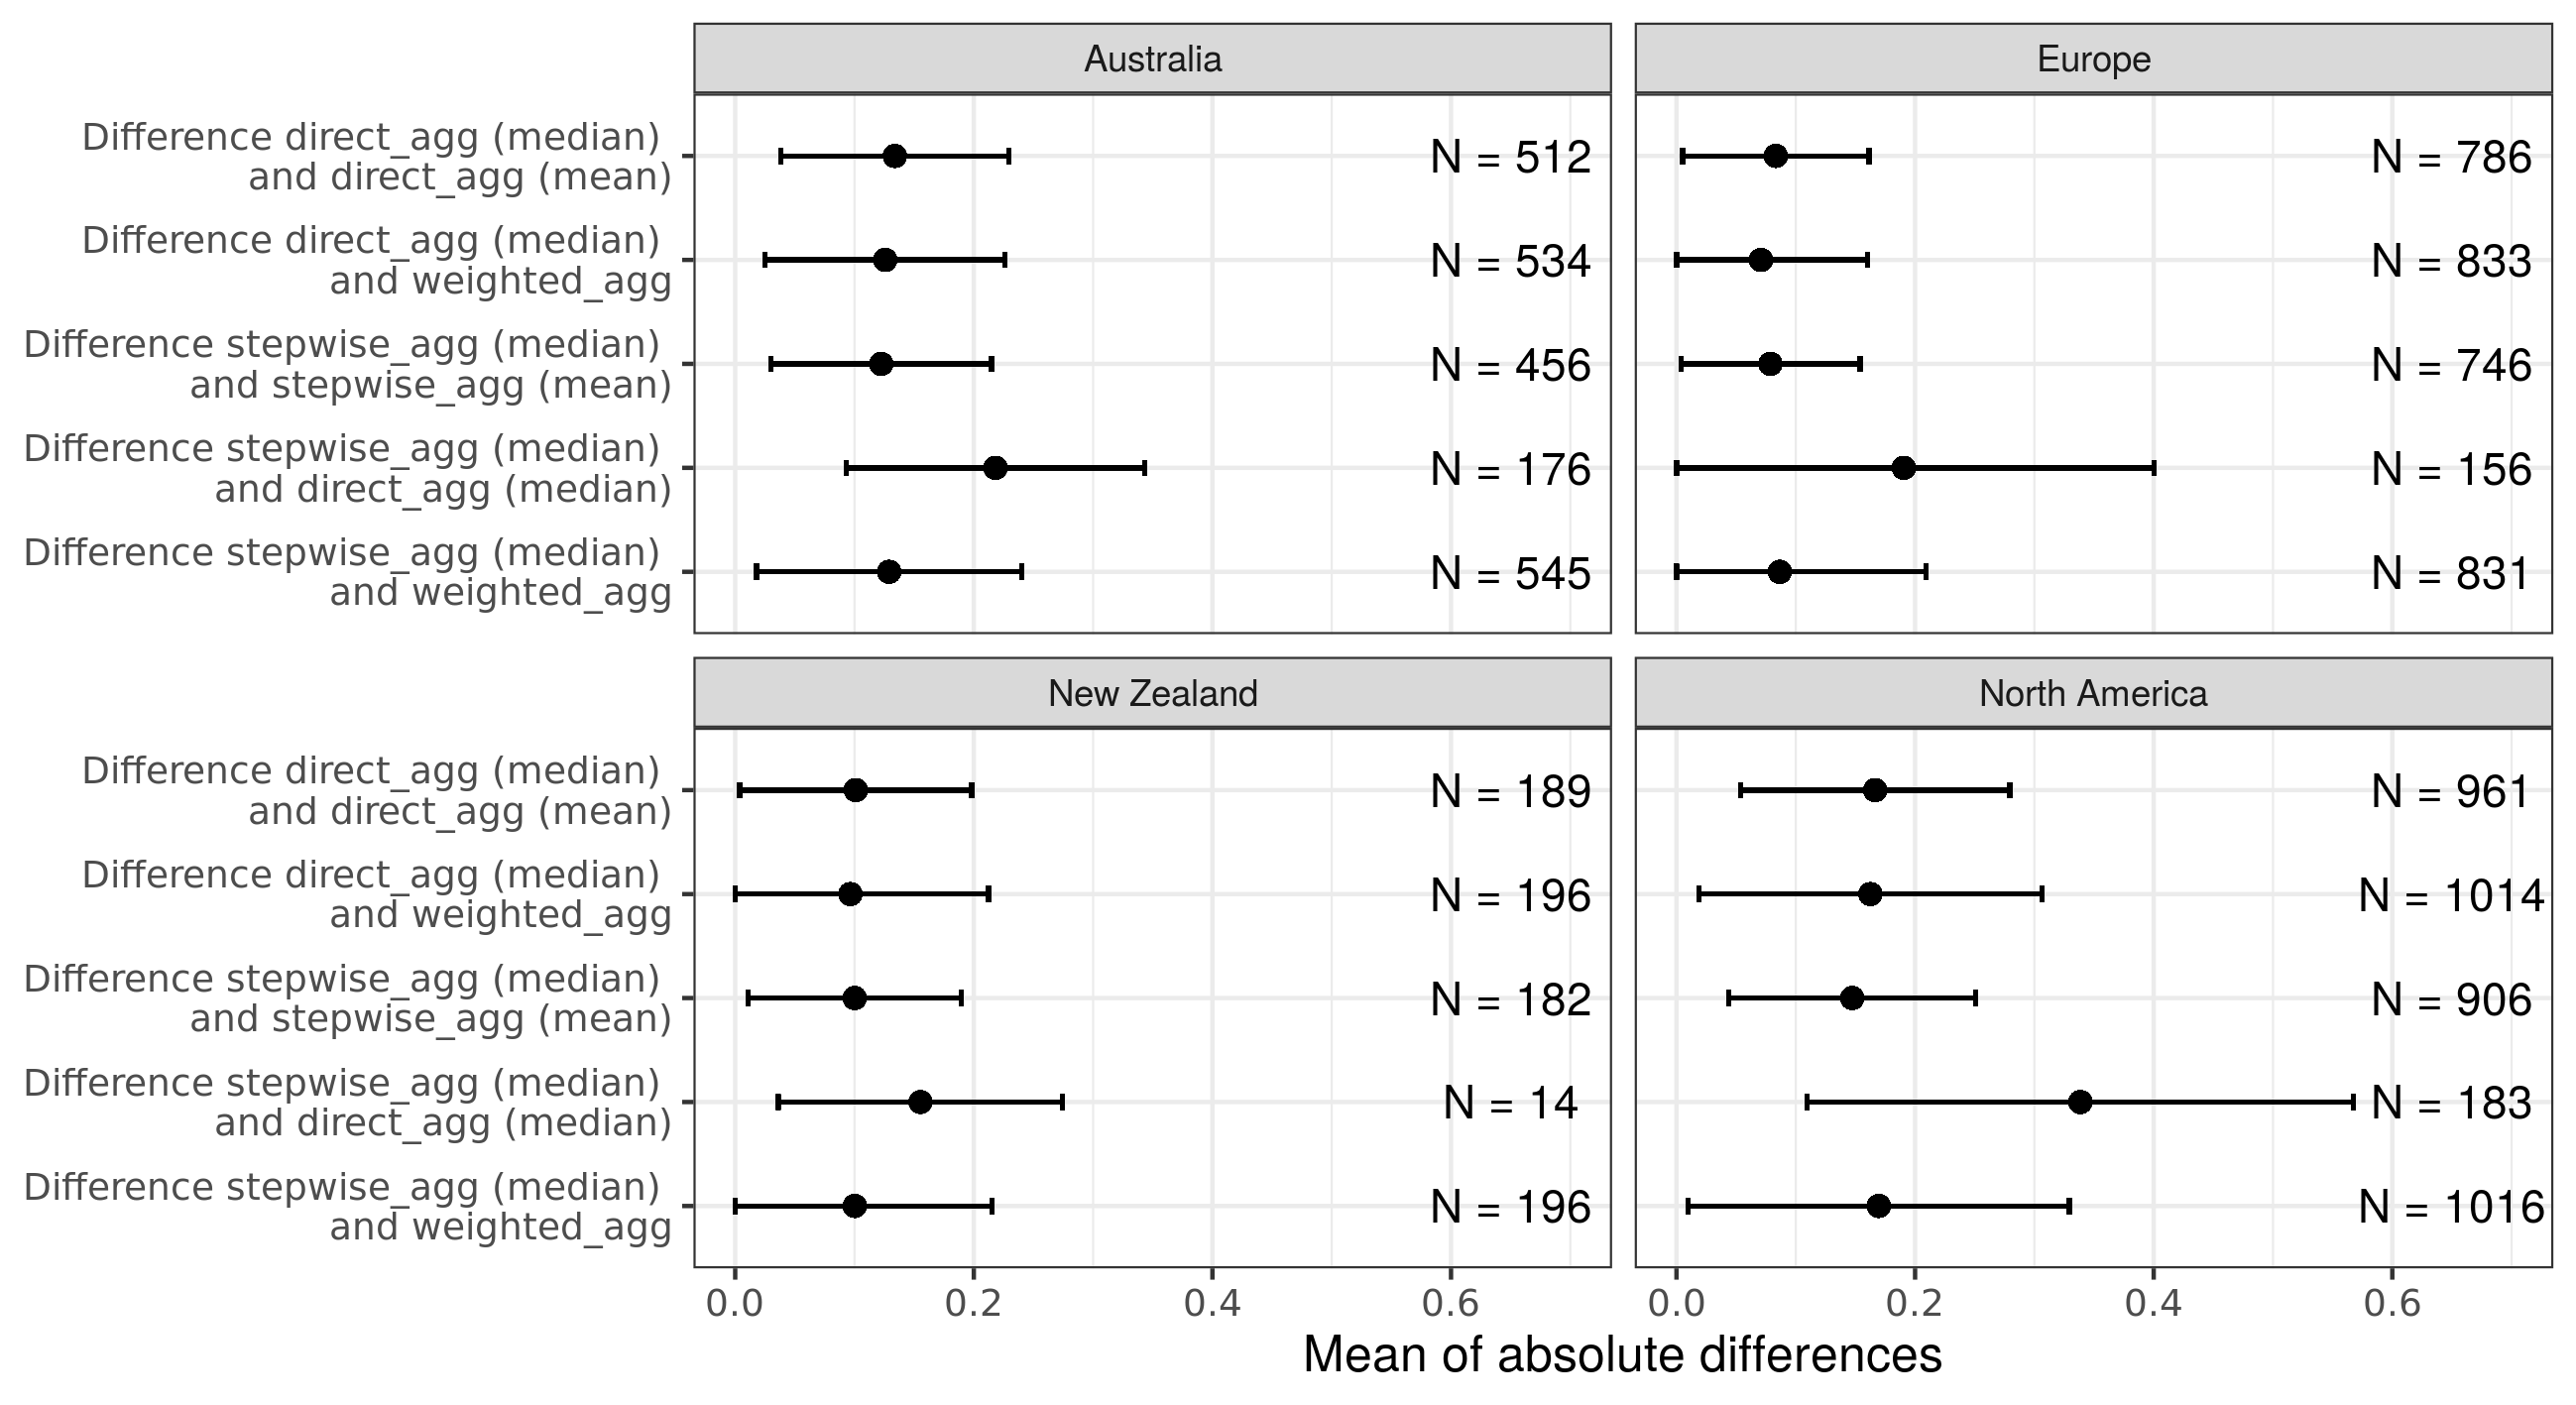
\includegraphics[width=16.5cm, height=10cm]{Comparison_trait_agg_methods.png}
    \caption{Means of absolute differences in trait affinities with standard deviations per region for all grouping features. Compared aggregation methods are displayed on the y-axis. N indicates the number of cases where differences occurred.}
\end{figure}

% \subsection*{Differences in trait affinities obtained by trait aggregation methods compared to traits assigned at family-level}
%? Cases where trait affinities aggregated through \textit{direct\_agg} differed more than 60 \% from trait affinities assigned at family-level by Chessman 2017

\newpage

\subsection*{Re-analysis of Szöcs et al. 2014 using harmonized and aggregated grouping features.}
\label{subsec:SI_szoecs_reanalysis}

\begin{figure}[H]
    \centering
    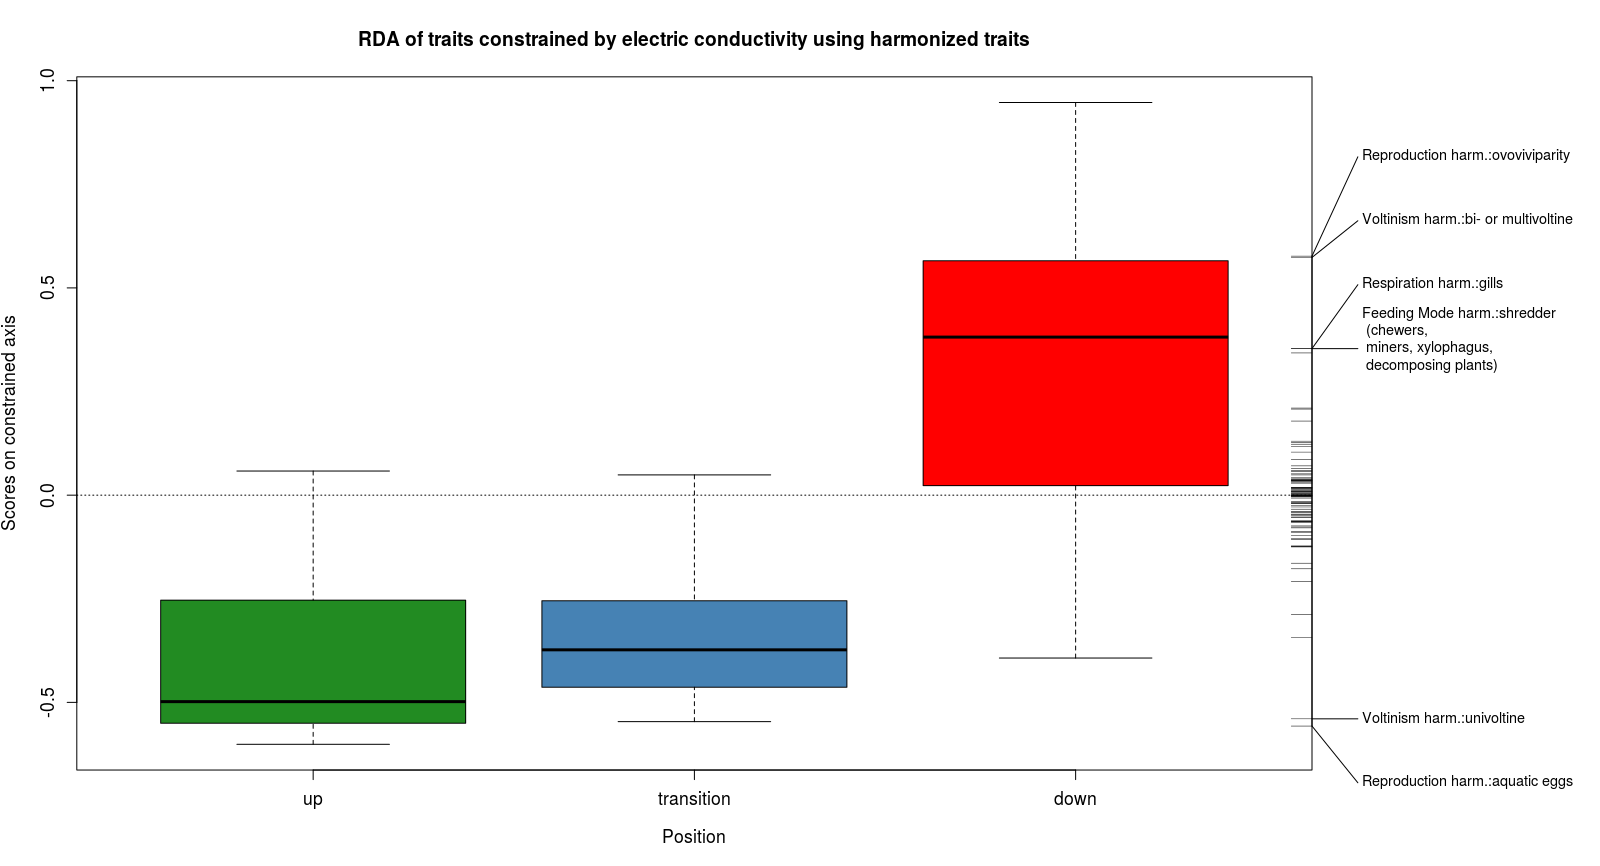
\includegraphics[width=16.5cm, height=10cm]{RDA_traits_harmonized.png}
    \caption{RDA of traits constrained by electric conductivity using harmonized grouping features. Boxplot of site scores along the conductivity axis ($31.44 \%$ explained variance, p = 0.001, 1000 permutations). Rug on the left indicates trait scores on the conductivity axis. Only traits with a mahalanobis distance greater than 5.02 were labeled in accordance to the procedure in Szöcs et al. 2014.
    } 
\end{figure}

\begin{figure}[H]
    \centering
    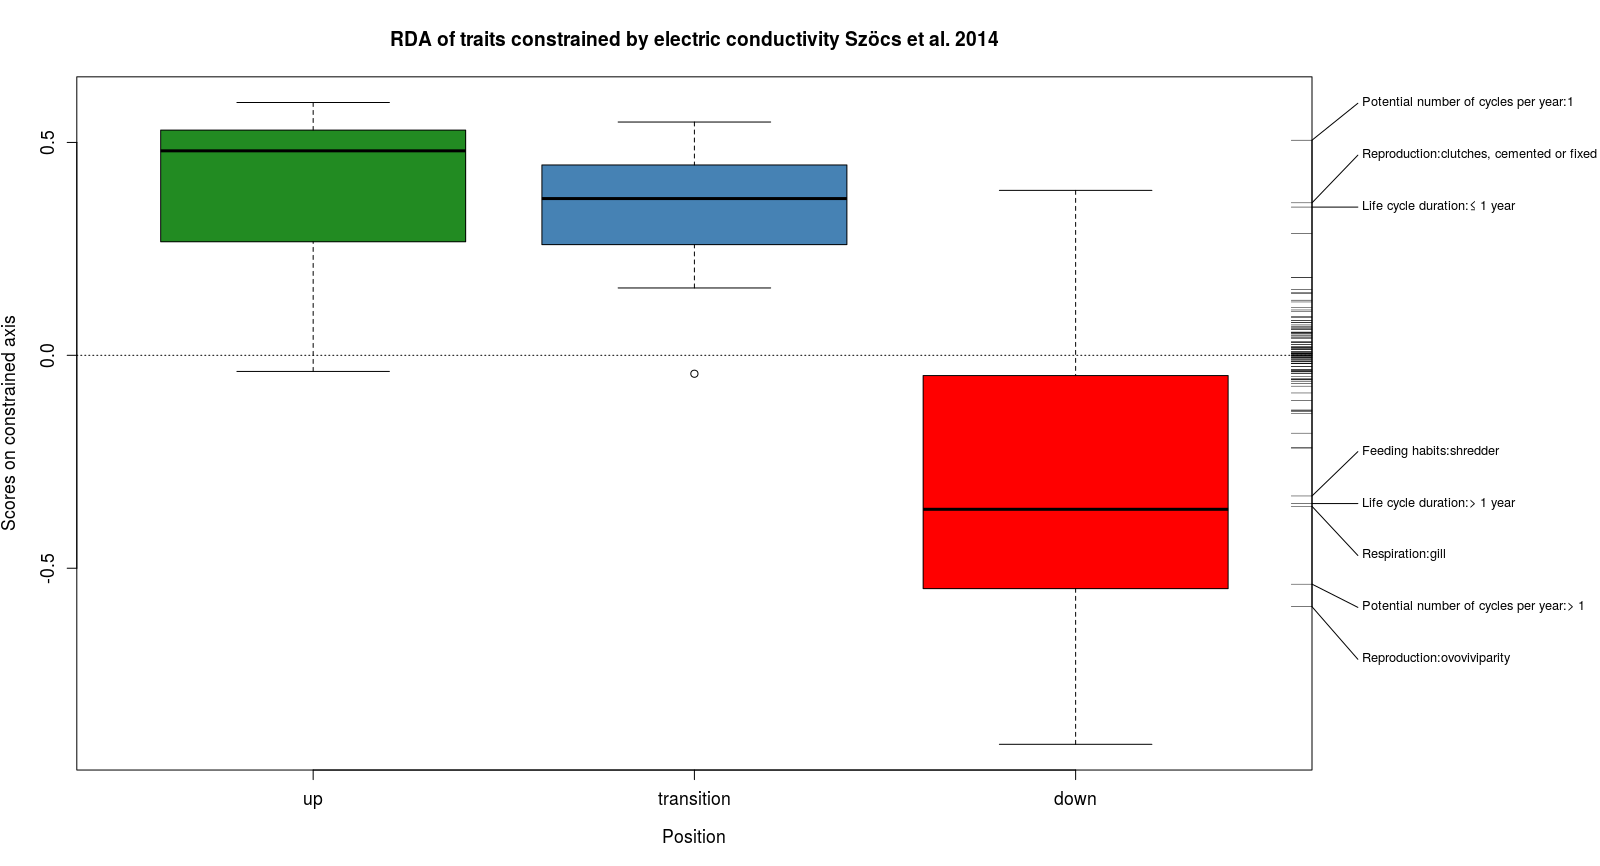
\includegraphics[width=16.5cm, height=10cm]{RDA_traits_Szoecs_2014.png}
    \caption{RDA of traits constrained by electric conductivity. Boxplot of site scores along the conductivity axis ($30.09 \%$ explained variance, p = 0.001, 1000 permutations). Rug on the left indicates trait scores on the conductivity axis. Only traits with a mahalanobis distance greater than 5.02 were labeled.
    } 
\end{figure}

\section*{Trait distribution along first RDA axis} 
\begin{figure}[H]
    \centering
    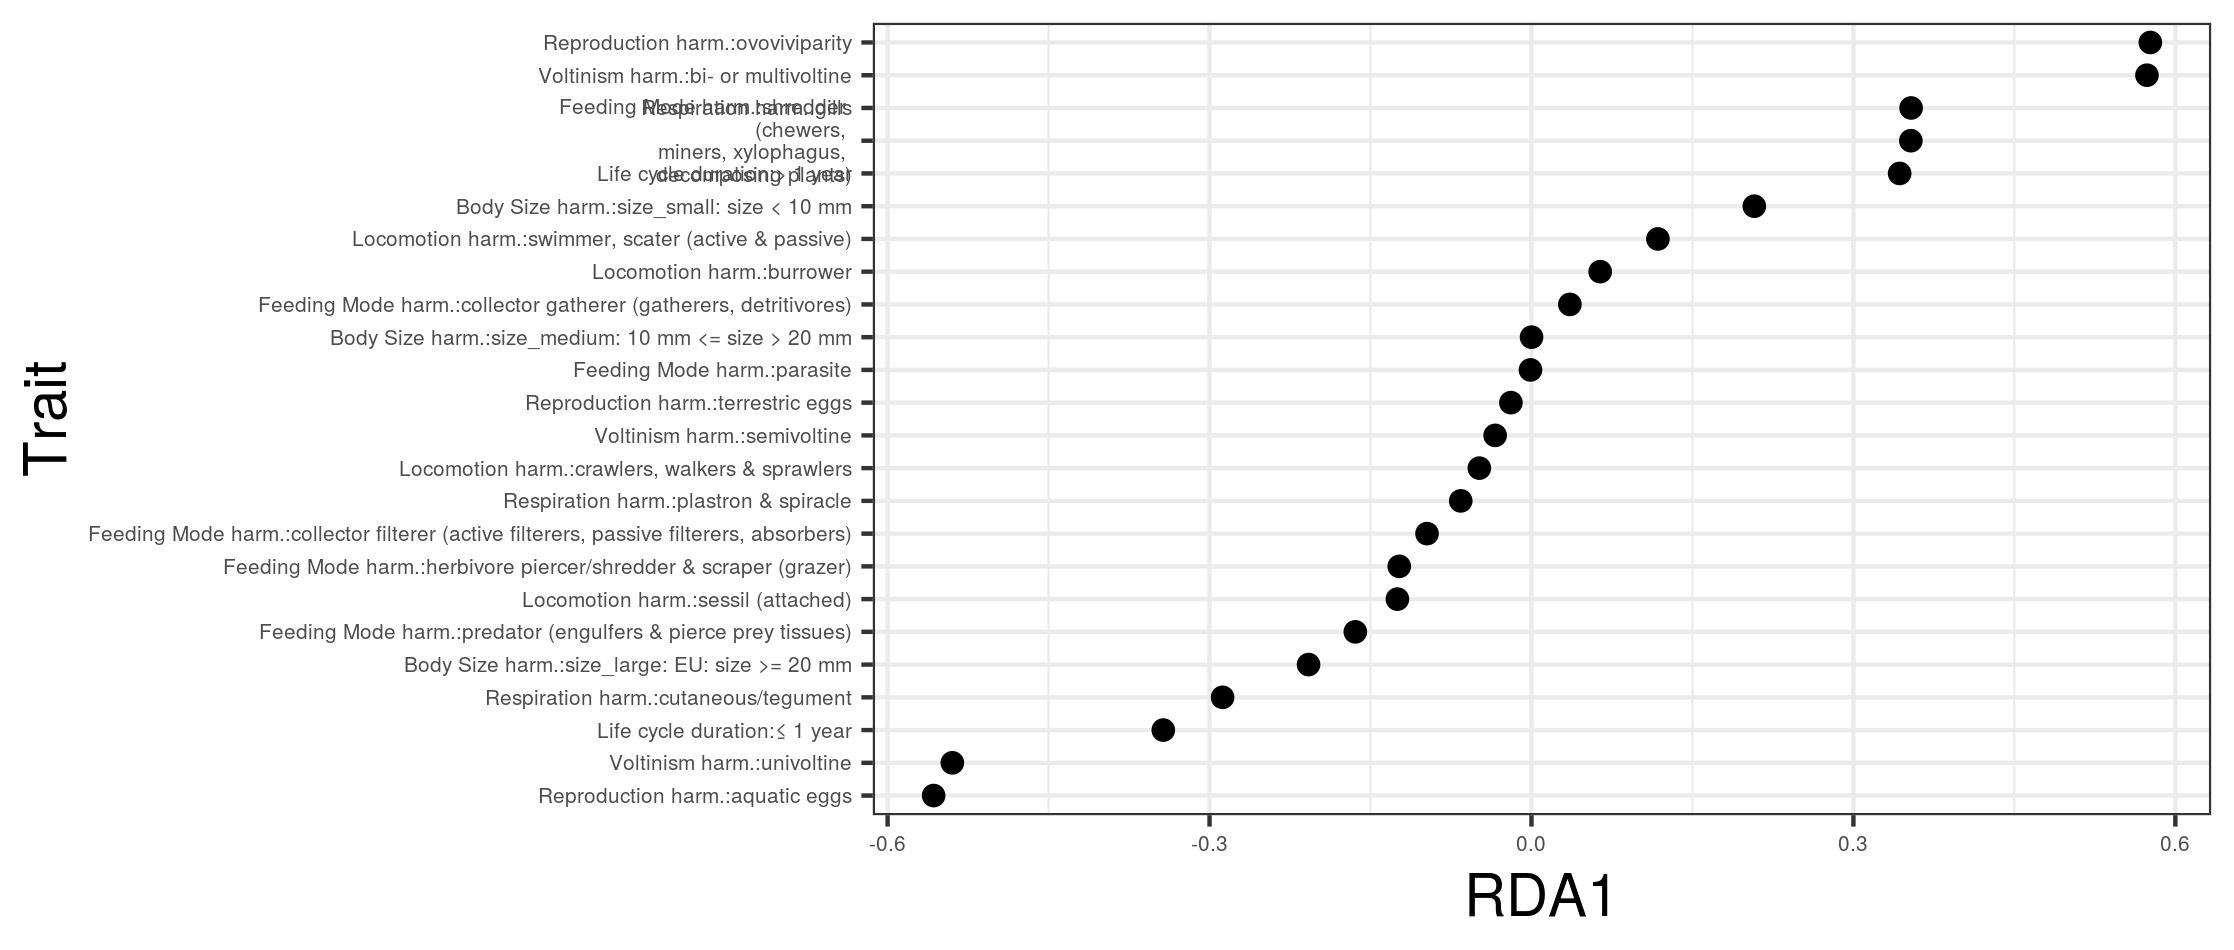
\includegraphics[width=17.5cm, height=10cm]{Trait_distrb_harmonized.png}
    \caption{Trait scores on the first RDA axis for harmonized traits and traits of the grouping feature \textit{life cycle duration}.
    } 
\end{figure}

\begin{figure}[H]
    \centering
    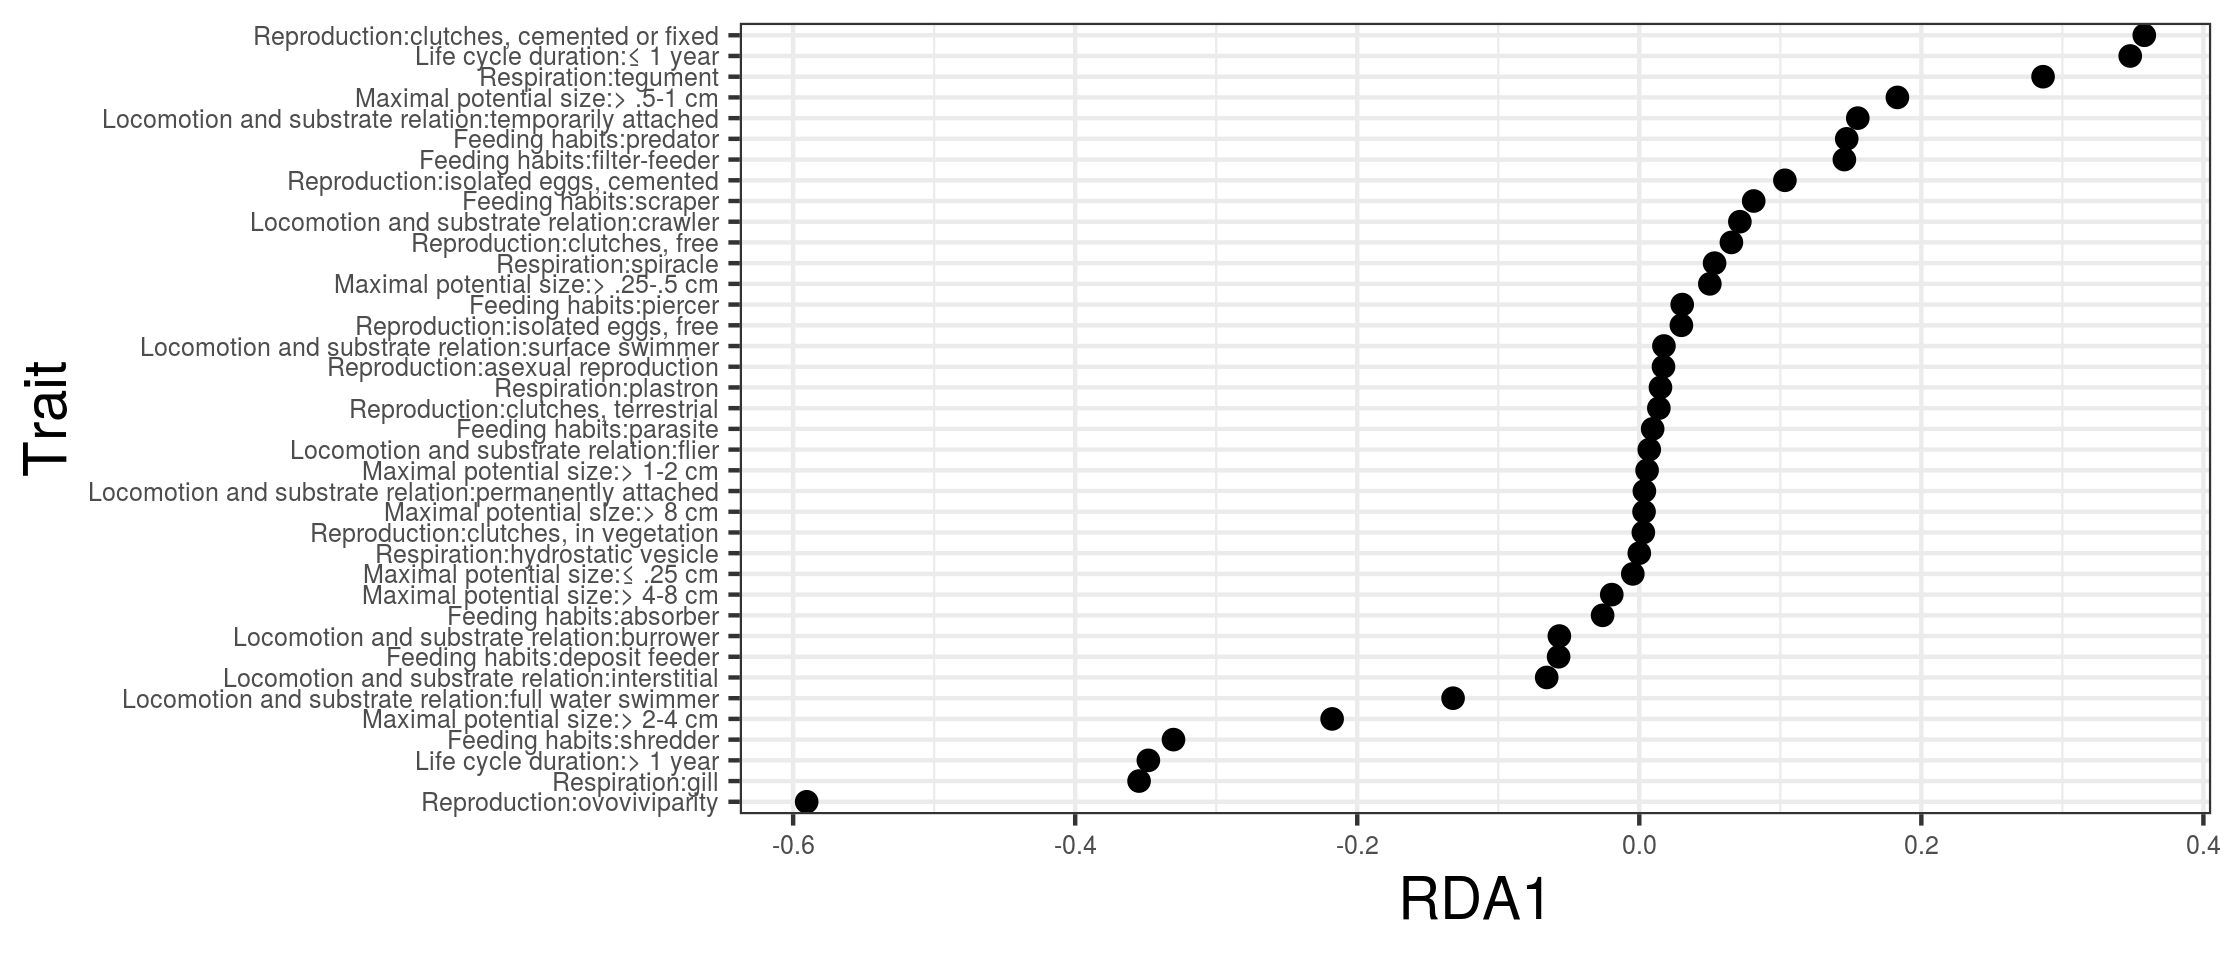
\includegraphics[width=17.5cm, height=10cm]{Trait_distrb_Szoecs_2014.png}
    \caption{Trait scores on the first RDA axis for the traits responding to high salinity in Szöcs et al. 2014
    .
    }
\end{figure}

\newpage
\section*{Linear models of trait proportions}
\textit{Linear models of trait proportions with harmonized traits:}
\begin{table}[ht]
    \centering
    \caption{Results of linear models for the four selected harmonized traits and life cycle duration $>$ 1 year. Trait proportions were logit transformed prior model building, estimates are on the logit scale. Although years were statistically not significant we kept this factor in the model to avoid temporal autocorrelation. Bold values indicate statistically significant effects (p $<$ 0.05).}
    \begin{tabular}{lccccc}
    \hline
    & \specialcell{Feeding mode:\\ shredder} & \specialcell{Life cycle duration:\\ $>$ 1 year} & \specialcell{Voltinism:\\ bi- or multivoltine} & \specialcell{Reproduction:\\ ovoviviparity} & \specialcell{Respiration:\\ gills} \\ 
    \hline
    Intercept ($=$ upstream) & \textbf{-1.041} & \textbf{-0.486} & 0.375* & \textbf{-0.823} & 0.092\\ 
    Downstream & \textbf{0.926} & \textbf{0.605} & \textbf{1.376} & \textbf{1.684} & \textbf{0.854}\\ 
    Downstream x 2008 & -0.117 & 0.106 & -0.235 & -0.088 & -0.317\\ 
    Downstream x 2009 & 0.030 & -0.056 & 0.001 & 0.245 & 0.180\\ 
    Year 2008 & -0.167 & -0.115 & 0.033 & -0.182 & -0.151\\ 
    Year 2009 & 0.175 & 0.086 & -0.088 & 0.246 & 0.141\\ 
    \hline
    \end{tabular}
    \textit{* p.value = 0.055}
\end{table}
\newline
\newline
\newline
\textit{Linear models of trait proportions Szöcs et al. 2014:}
\begin{table}[ht]
    \centering
    \caption{Results of linear models for the five selected traits for Szöcs et al. 2014. Trait proportions were logit transformed prior model building, estimates are on the logit scale.
    Although years were statistically not significant we kept this factor in the model to avoid temporal autocorrelation. Bold values indicate statistically
    significant effects (p $<$ 0.05).}
    \begin{tabular}{lccccc}
    \hline
    & \specialcell{Feeding habits:\\ shredder} & \specialcell{Life cycle duration:\\ $>$ 1 year} & \specialcell {Cycles per year:\\ $>$ 1} & \specialcell{Reproduction:\\ ovoviviparity} & \specialcell{Respiration:\\ gills} \\ 
    \hline
    Intercept ($=$ upstream) & \textbf{-0.853} & \textbf{-0.478} & \textbf{0.603} & \textbf{-0.838} & 0.111 \\ 
    Downstream & \textbf{0.819} & \textbf{0.594} & \textbf{1.297} & \textbf{1.679} & \textbf{0.839} \\ 
    Downstream x 2008 & -0.155 & 0.102 & -0.227 & -0.070 & -0.314 \\ 
    Downstream x 2009 & 0.073 & -0.053 & -0.020 & 0.248 & 0.176 \\ 
    Year 2008 & -0.122 & -0.112 & 0.026 & -0.192 & -0.154 \\ 
    Year 2009 & 0.167 & 0.084 & -0.104 & 0.250 & 0.139 \\ 
    \hline
    \end{tabular} 
\end{table}


\section*{Trait proportions over time}
\begin{figure}[H]
    \centering
    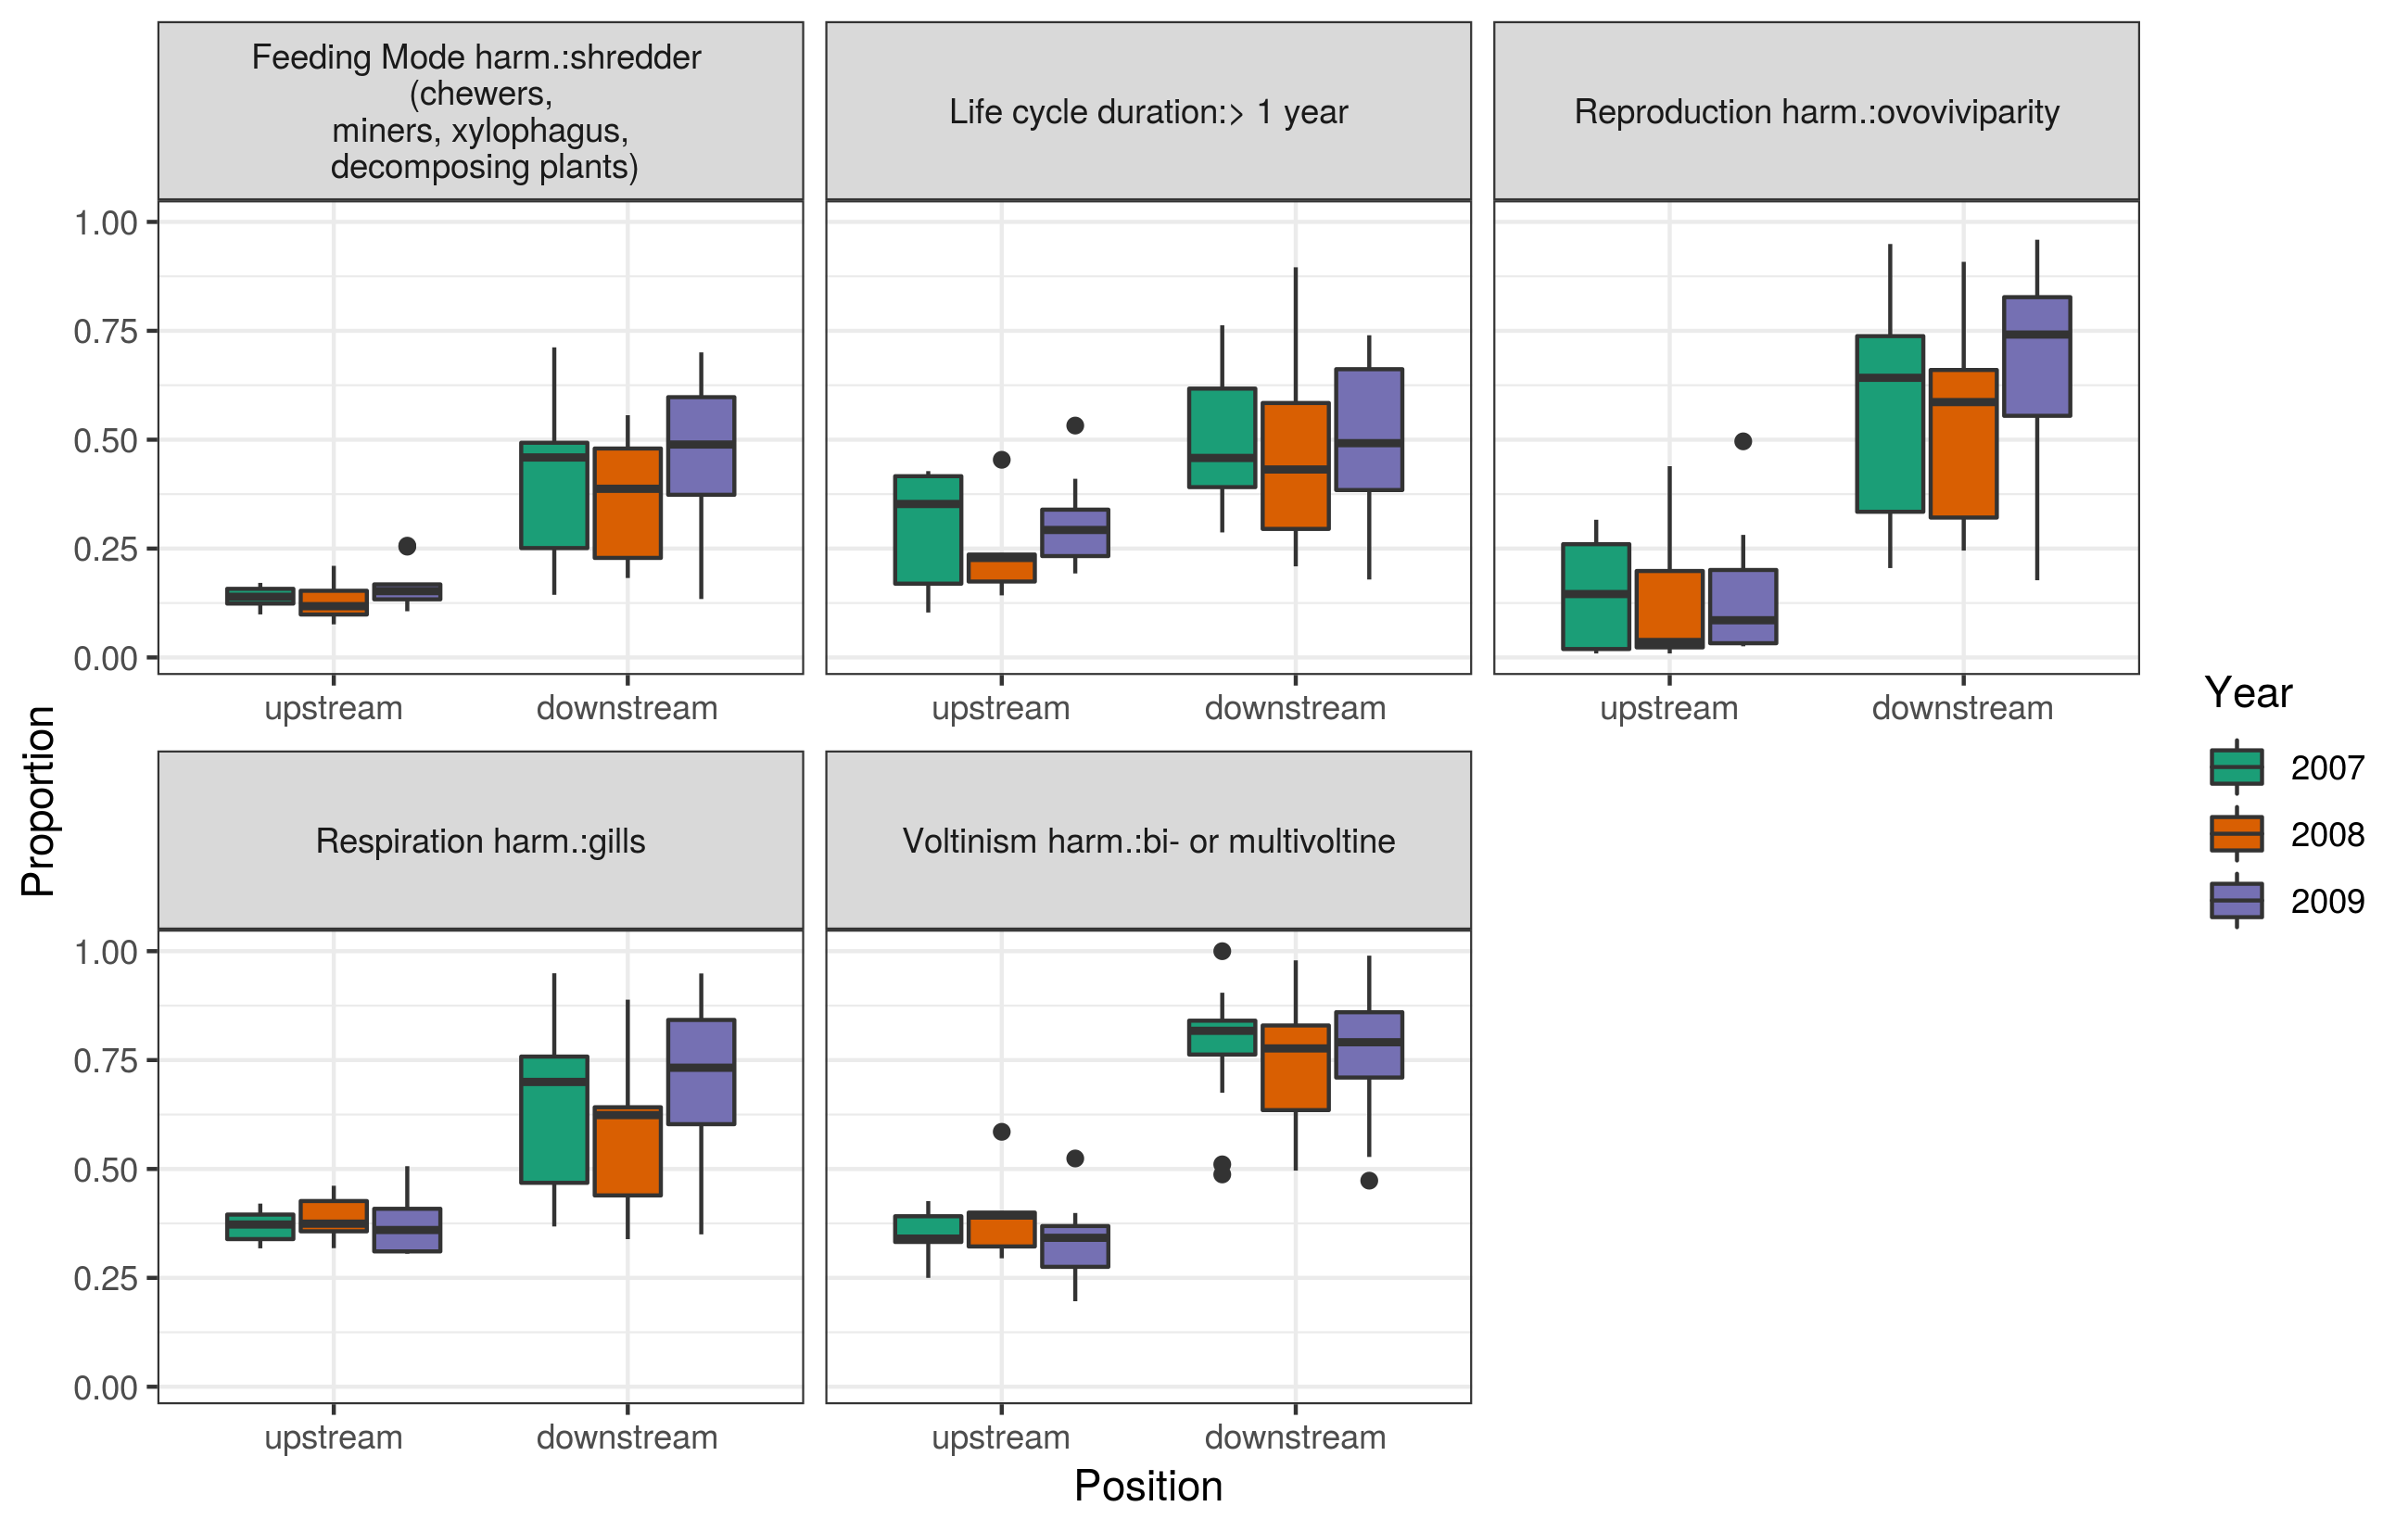
\includegraphics[width=16.5cm, height=10cm]{Trait_proportion_harmonized.png}
    \caption{Proportions for the four harmonized traits that have been promoted by salinization and life cycle duration $>$ 1 year for down- and upstream sites.
    } 
\end{figure}

% Trait proportions over time
\begin{figure}[H]
    \centering
    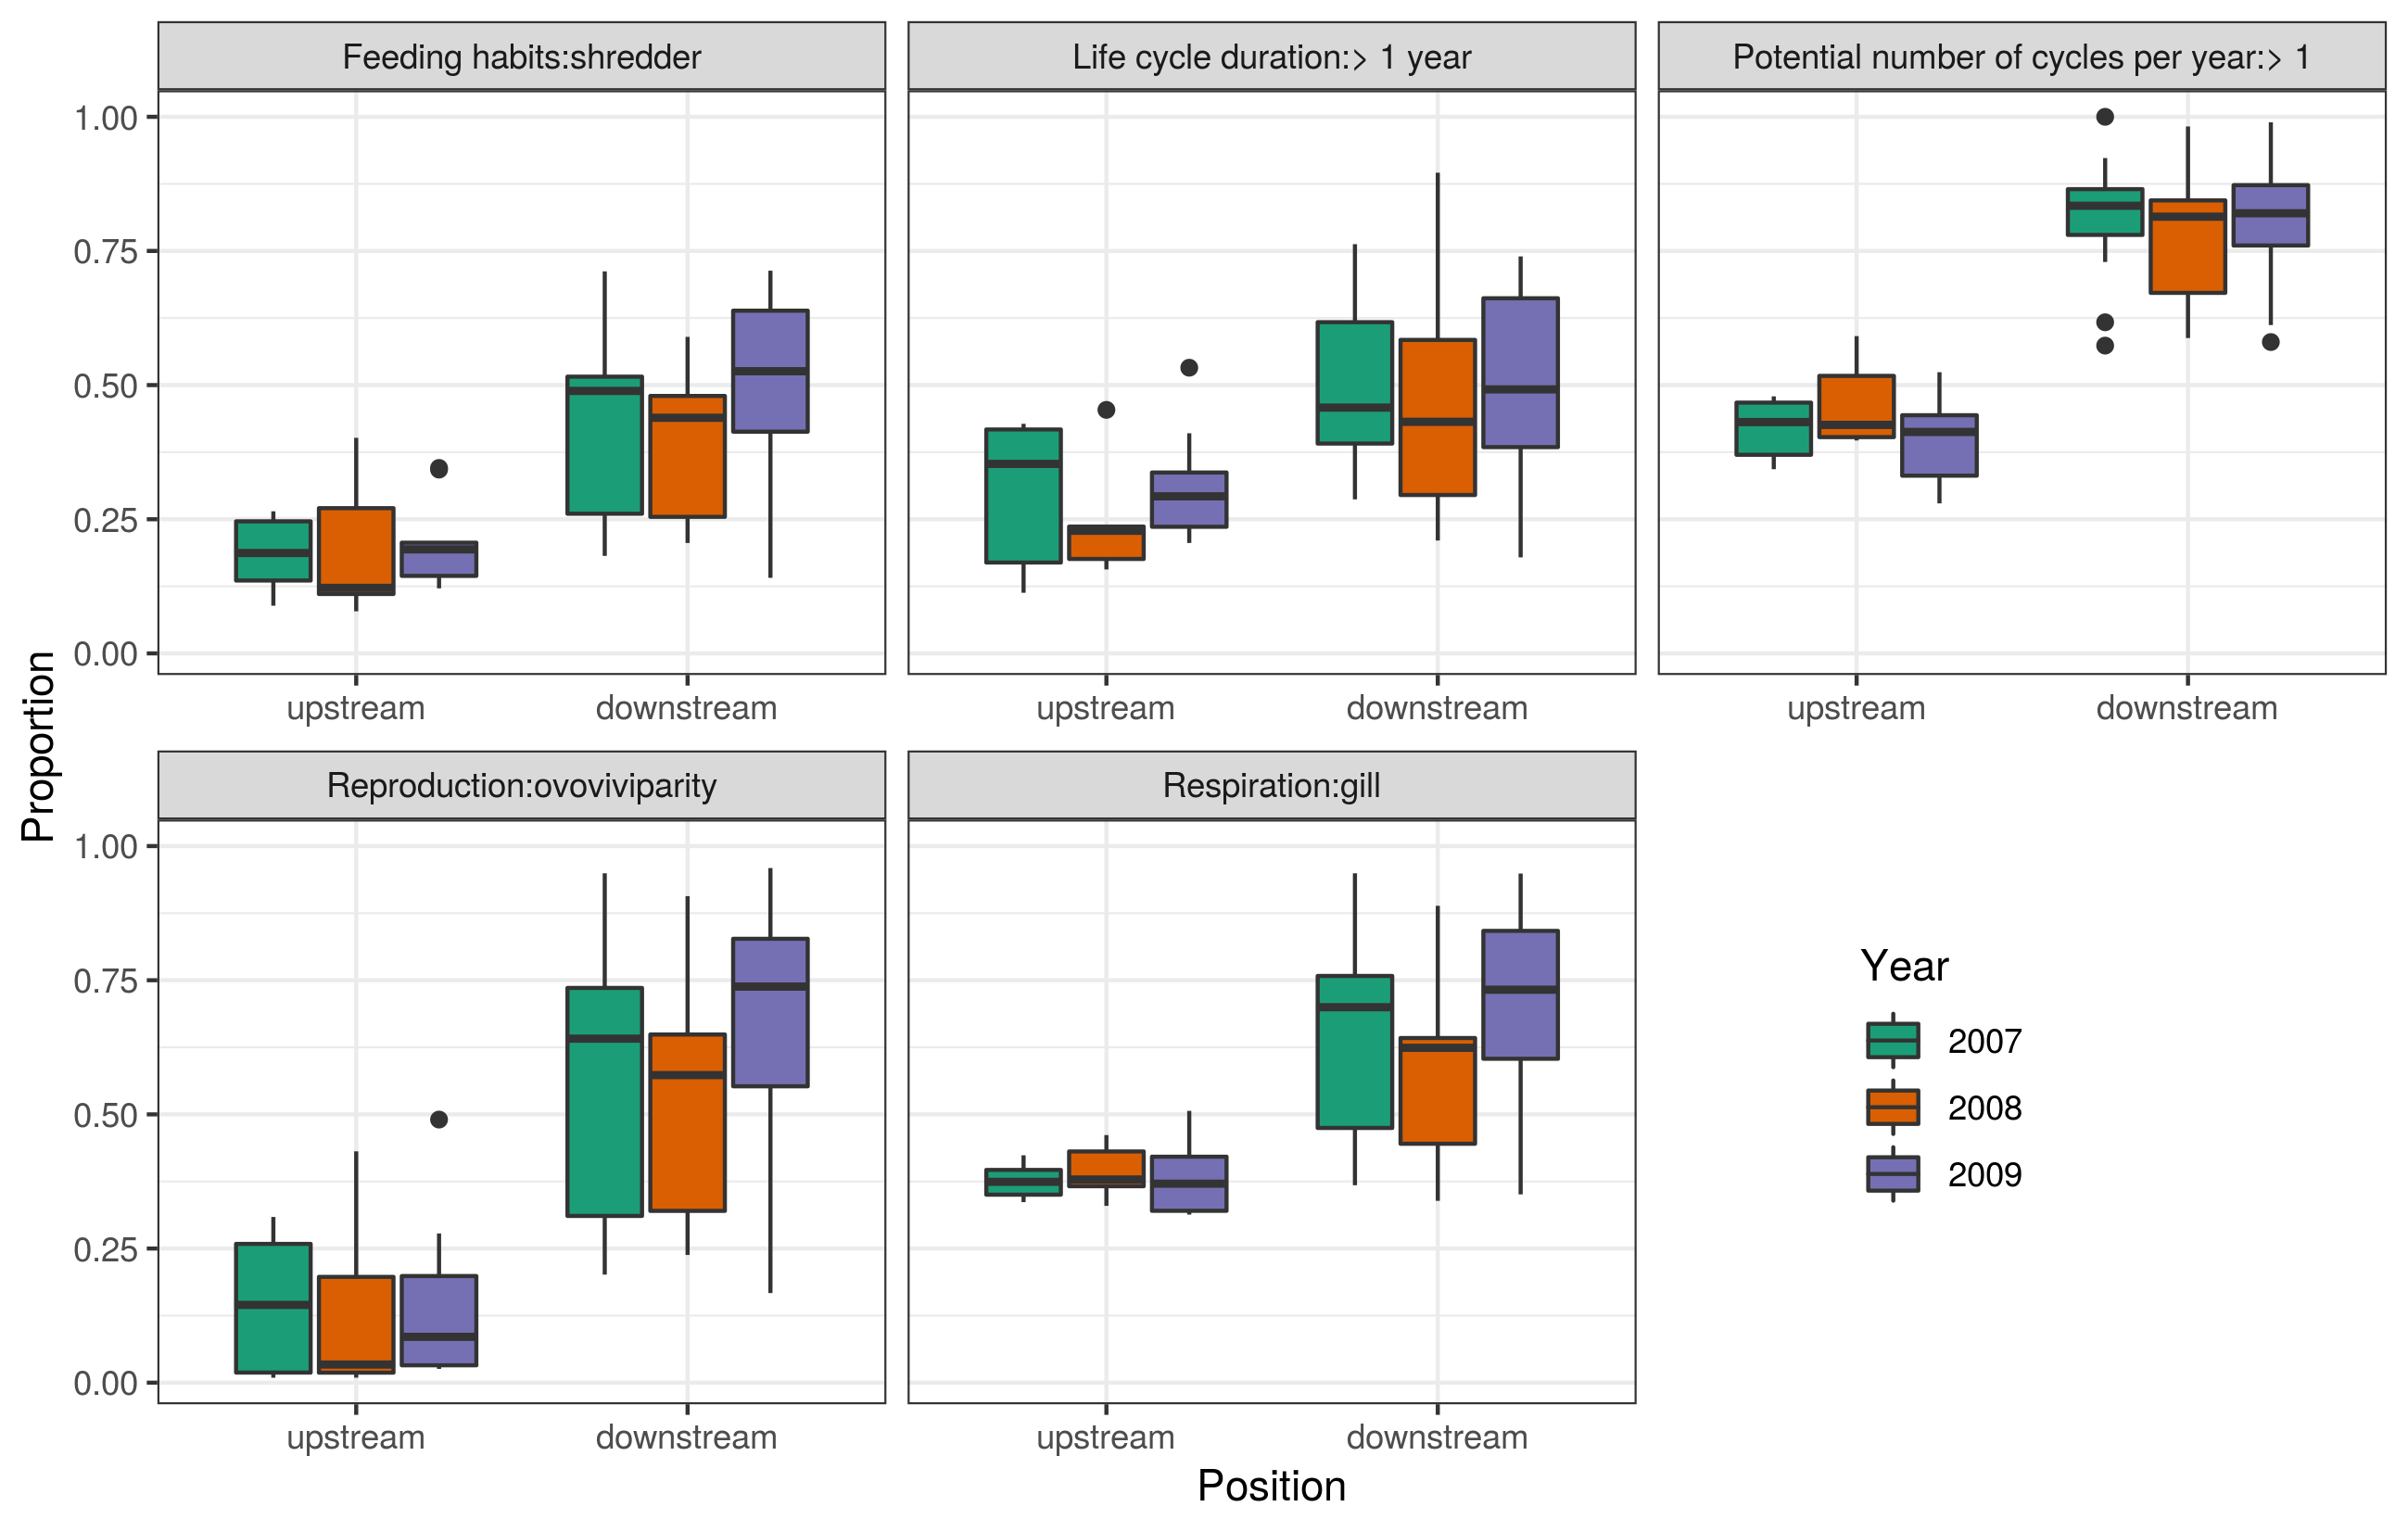
\includegraphics[width=16.5cm, height=10cm]{Trait_proportion_Szoecs_2014.png}
    \caption{Proportions for five selected traits for down- and upstream sites (traits that have been promoted by salinization) from Szöcs et al. 2014.} 
\end{figure}

\newpage

\section*{Harmonization of the European trait databases}
\label{sec:SI_harmonization_EU}

% \cellcolor{blue!25}
\begin{longtable}{lll|l}
%\begin{table}[ht]
%    \centering
    \caption{Representation of traits per grouping feature and their harmonization for the European trait databases. The color coding indicates traits that have been harmonized. Cyan colored traits have not been used because they either represented ambiguous traits or traits that were not compatible with the traits of the other databases. Harmonization was done by assigning the maximum affinity of the allocated traits for the respective taxa to the harmonized trait.}
    \endfirsthead
    \endhead
    %\begin{tabular}{llll}
    \hline
    Grouping feature & Freshwater ecology & Tachet & Harmonized traits \\ 
    \hline
    \hline
    Voltinism & Semivoltine & Semivoltine & Semivoltine \\ 
    Voltinism & Univoltine & Univoltine & Univoltine \\ 
    \rowcolor{gray!25}
    Voltinism & Bivoltine & Polyvoltine & Bi/Multivoltine \\ 
    \cellcolor{gray!25}Voltinism & \cellcolor{gray!25}Trivoltine &  &  \\ 
    \cellcolor{gray!25}Voltinism & \cellcolor{gray!25}Multivoltine &  &  \\ 
    \cellcolor{gray!25}Voltinism & \cellcolor{gray!25}Flexible &  &  \\ 
    \rowcolor{blue!25}
    \cellcolor{blue!25}Feeding Mode & \cellcolor{blue!25}Shredder & Shredder & Shredder \\ 
    \cellcolor{blue!25}Feeding Mode & \cellcolor{blue!25}Miner & Deposit-feeder & Gatherer \\ 
    \cellcolor{blue!25}Feeding Mode & \cellcolor{blue!25}Xylophagus & \cellcolor{blue!50}Absorber & \cellcolor{blue!50}Filterer \\ 
    Feeding Mode & Gatherer & \cellcolor{blue!50}Filter-feeder & Herbivore \\ 
    \cellcolor{blue!50}Feeding Mode & \cellcolor{blue!50}Active filterer & Scraper & Predator \\ 
    \cellcolor{blue!50}Feeding Mode & \cellcolor{blue!50}Passive filterer & Predator & Parasite \\ 
    Feeding Mode & Grazer & Parasite &  \\ 
    Feeding Mode & Predator & \textit{Piercer (plants or animals)} \textsuperscript{\textit{a}} &  \\ 
    Feeding Mode & Parasite &  &  \\ 
    \color{cyan}Feeding Mode & \color{cyan}Other &  &  \\ 
    \hline
    \rowcolor{green!15}
    Locomotion & Swimming/scating & Surface swimmer & Swimmer \\ 
    \cellcolor{green!15}Locomotion & \cellcolor{green!15}Swimming/diving & \cellcolor{green!15}Full water swimmer & \cellcolor{green!50}Burrower \\ 
    \cellcolor{green!50}Locomotion & \cellcolor{green!50}Burrowing/boring & \cellcolor{green!50}Burrower & Crawler \\
    Locomotion &  & \cellcolor{green!50}Interstitial & \cellcolor{green!95}Sessil \\
    Locomotion & Sprawling/walking & Crawler &  \\ 
    \cellcolor{green!95}Locomotion & \cellcolor{green!95}(semi) sessil & \cellcolor{green!95}Temporarily attachted &  \\ 
    \color{cyan}Locomotion & \color{cyan}Other & \cellcolor{green!95}Permanently attached &  \\ 
    \color{cyan}Locomotion &  & \color{cyan}Flier &  \\
    \hline
    Respiration & Tegument & Tegument & Tegument \\ 
    Respiration & Gill & Gill & Gills \\ 
    \rowcolor{orange!25}
    Respiration & Plastron & Plastron & Plastron, spiracle \\ 
    \cellcolor{orange!25}Respiration & \cellcolor{orange!25}Spiracle (aerial) & \cellcolor{orange!25}Spiracle (aerial) &  \\ 
    \color{cyan}Respiration & \color{cyan}Hydrostatic vesicle & \color{cyan}Hydrostatic vesicle (aerial) &  \\ 
    \color{cyan}Respiration & \color{cyan}Tapping (air stores of aq. plants) &  &  \\ 
    \color{cyan}Respiration & \color{cyan}Excursion/Extension (to surface) &  &  \\ 
    \hline
    Body size &  & $<$= 0.25cm & Small ($<$ 1 cm) \\ 
    Body size &  & $>$ 0.25 - 0.5cm & Medium ($>$= 1cm - 2 cm) \\ 
    Body size &  & $>$ 0.5- 1cm & Large ($>$= 2 cm) \\ 
    Body size &  & $>$ 1 – 2 cm &  \\ 
    Body size &  & 2 – 4 cm &  \\ 
    Body size &  & 4 – 8 cm &  \\ 
    Body size &  & $>$ 8 cm &  \\ 
    \hline
    Reproduction & ovovivipar & ovoviviparity & ovoviviparity \\ 
    \rowcolor{purple!25}
    Reproduction & free isolated eggs & isolated eggs, free & aquatic eggs \\ 
    \cellcolor{purple!25}Reproduction & \cellcolor{purple!25}cemented isolated eggs & \cellcolor{purple!25}isolated eggs, cemented & terrestrial eggs \\
    \cellcolor{purple!25}Reproduction & \cellcolor{purple!25}fixed clutches & \cellcolor{purple!25}clutches, cemented or fixed &  \\ 
    \cellcolor{purple!25}Reproduction & \cellcolor{purple!25}free clutches & \cellcolor{purple!25}clutches, free &  \\ 
    \cellcolor{purple!25}Reproduction & \cellcolor{purple!25}clutches in vegetation & \cellcolor{purple!25}clutches, in vegetation &  \\ 
    Reproduction & terrestrial clutches & clutches, terrestrial &  \\ 
    \color{cyan}Reproduction & \color{cyan}asexual & \color{cyan}asexual reproduction &  \\ 
    \color{cyan}Reproduction & \color{cyan}parasitic &  &  \\ 
    \hline
    %\end{tabular}
%\end{table}
\end{longtable}
\begin{minipage}{\linewidth}\small
    \textit{a} Taxa exhibiting this trait have been assigned to predators or herbivores based on a classification by Philippe Usseglio-Polatera.
\end{minipage}

%%%%%%%%%%%%%%%%%%%% OLD %%%%%%%%%%%%%%%%%%%%%%%%%%%%%%%%%%%%%%%%%%
% \subsection*{Deviance in trait affinities between \textit{stepwise\_agg} and \textit{direct\_agg (median)}}

% \begin{figure}[H]
%     \centering
%     \includegraphics[width=16.5cm, height=10cm]{Deviances_stepwise_dir_overview.png}
%     \caption{Affinity deviances for all deviating cases between the \textit{stepwise\_agg} and \textit{direct\_agg}, see section \ref{sec:dev_stepwise_direct_agg}.}
%     \label{fig:stepwise_dir_agg}
% \end{figure}


% \subsection*{Comparison of trait affinity values \textit{direct\_agg} using median or mean}

% \begin{figure}[H]
%     \centering
%     \includegraphics[width=16.5cm, height=10cm]{Deviances_dir_median_mean_overview.png}
%     \caption{Affinity deviances for all deviating cases between the \textit{direct\_agg (median)} and \textit{direct\_agg (mean)}, see section \ref{sec:comp_direct_agg_median_mean}.}
%     \label{fig:dir_agg_median_mean}
% \end{figure}

% \subsection*{Deviances in trait affinities between \textit{direct\_agg} and \textit{weighted\_agg}}

% \begin{figure}[H]
%     \centering
%     \includegraphics[width=16.5cm, height=10cm]{Deviances_dir_weighted_overview.png}
%     \caption{Affinity deviances for all deviating cases of comparisons between the \textit{direct\_agg (median)} and \textit{direct\_agg (mean)} with \textit{weighted\_agg}, see section \ref{sec:dev_dir_agg_weighted}.}
%     \label{fig:dir_agg_median_mean_weighted}
% \end{figure}

\end{document}